\section{Theorie}
\label{sec:theory}
Der LHCb Detektor ist einer der vier großen Detektoren am Large Hadron Collider (LHC) der European Organization for Nuclear Research (CERN).
Er untersuchtProton-Proton-Kollisionen, 
die am LHC bei einer Schwerpunktsenergie von bis zu $13.6$ TeV stattfinden \cite{Anleitung}.
Dafür ist der LHCb Detektor unteranderem mit einem Spektrometersystem ausgestattet,
das es ermöglicht den Impuls von geladenen Teilchen zu bestimmen.
Die dafür benötigte Hauptspurenkammer ist der Scintillating Fibre Tracker (SciFi).
Er dedektiert die geleadenen Teilchen durch in szintilierende Fasern entstehende Photonen.
Das verhalten der Photonen in den Fasern soll in Kapittel~\ref{sec:Analysis} charakterisiert werden.
Dazu wird nachdem in Abschnit~\ref{sec:LHCb} und \ref{sec:SciFi} der LHCb Detektor und besonders der SciFi Detektor genauer beschrieben wurde,
in Abschnitt~\ref{sec:szintilierende_Fasern} die Funktionsweise der szintilierenden Fasern erklärt (Abschnitt~\ref{sec:mechanismus}) und das verhalten der Photonen Mathematisch beschrieben (Abschnitt~\ref{sec:transport}).



\subsection{Der LHCb Detektor}
\label{sec:LHCb}
\begin{figure}[h]
	\centering
	
\includegraphics[width=\textwidth]{content/Figures/LHCb.png}
	\caption[Schematische Darstellung des LHCb Upgrade 2 Detektors.]{Schematische Darstellung eines Querschnittes des LHCb Upgrade 2 Detektors \cite{TDR}.}
	\label{fig:LHCb}
\end{figure}
Der LHCb-Detektor ist als einarmiger Vorwärtsspektrometer konstruiert, 
da die $b$- $\bar{b}$-Paare bei den $pp$-Kollisionen überwiegend unter einem kleinen Winkel relativ zur Strahlachse produziert werden.
Daher sind die daraus entstehenden Hadronen in dieselbe Richtung geboostet \cite{bbangles}.

In Abbildung \ref{fig:LHCb} wird der Querschnitt des LHCb Detektors dargestellt.
Der \textit{Vertex-Locator} (VELO) dient der Identifizierung und Unterscheidung der primären und sekundären Vertices der Zerfälle.
Da diese nur wenige Millimeter auseinander liegen,
befindet sich der VELO direkt am Interaktionspunkt.
Zusammen mit dem \textit{Upstream Tracker} (UT), 
dem \textit{Dipolmagneten} und dem \textit{SciFi Detektor} bildet der VELO das Spektrometersystem des LHCbs.
Dieses dient der Rekonstruktion von Teilchenspuren und der Bestimmung des Impulses.
Der durch die Ablenkung der Teilchen in einem Magnetfeld bestimmt werden kann.

Die Detektoren \textit{RICH1}, \textit{RICH2}, \textit{ECAL}, \textit{Hcal} und die Myon Stationen \textit{M2} bis \textit{M5} dienen der Teilchenidentifikation.
Der Schwerpunkt liegt hier in der Unterscheidung von Elektronen, Photonen, Kaonen und Protonen,
da sie häufige Zerfallsprodukte von $b$-Hadronen sind \cite{TDR}.



\subsection{Der SciFi Detektor}
\label{sec:SciFi}
Der SciFi Detektor befindte sich direkt hinter dem Dipolmagnet des LHCb Detektors und ist damit unerlässlich für die rekonstruktion von Teilchenspuren, 
die durch den Magneten abgelenkt werden.
Er bedeckt eine sensible Fläche von $340$ m$^2$ und besteht aus mehr als $10000$ km szintilierenden Fasern.
Die verwendeten Fasern haben einen Durchmesser von \SI{250}{\micro\meter} und werden in sechs gegeneinander versetzten Schichten zu einer kompakten Struktur aufgewickelt. 
Auf diese Weise entstehen Fasermatten mit einer Länge von 2,4m und einer Breite von 13cm. 
Eine Stirnseite der Matten ist mit einem Spiegel ausgestattet, 
der das entstehende Szintillationslicht zurück in Richtung des gegenüberliegenden Endes lenkt, 
an dem sich die Ausleseelektronik befindet. 
Jeweils acht dieser Matten werden zu größeren Einheiten zusammengefasst, die eine Gesamtbreite von 0,5m aufweisen.
Aus diesen Einheiten bestehen dann die drei Detektorebenen des SciFi Detektors, 
die jeweils 12m lang sind und eine Breite von 4,8m aufweisen.

Jede der Detektorebenen besteht aus vier Schichten, 
die in einer x-u-v-x Anordnung angeordnet sind.
\begin{figure}
    \centering
    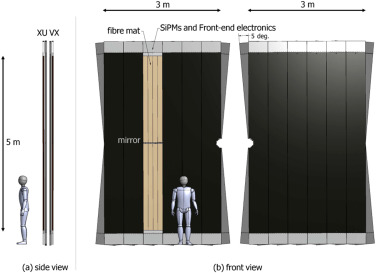
\includegraphics[width=0.8\textwidth]{content/Figures/Station.jpg}
    \caption[Schematische Darstellung einer Station des SciFi Detektors.]{Schematische Darstellung einer Station des SciFi Detektors \cite{Gruber2020}.}
    \label{fig:SciFi}
\end{figure}
Die x-Schichten sind parallel zur Strahlachse ausgerichtet,
während die u- und v-Schichten um \SI{5}{\degree} gegenüber der x-Achse geneigt sind.
Diese Anordnung ermöglicht es, 
die Position der durch die Fasern detektierten Teilchen
sowohl in der horizontalen als auch in der vertikalen Richtung zu bestimmen.
Eine solche Station ist in Abbildung~\ref{fig:SciFi} dargestellt.

Am ende der Fasern befindet sich die Ausleseelektronik,
die aus sogenannten Silicon Photomultipliern (SiPMs) besteht.
Wenn ein geladenes Teilchen die Fasern durchquert,
entstehen in den Fasern Photonen, die von den SiPMs detektiert werden \cite{Anleitung}.



\subsection{Szintilierende Fasern}
\label{sec:szintilierende_Fasern}
Damit die durch den in Abschnitt~\ref{sec:mechanismus} beschriebenen Mechanismus entstehenden Photonen die SiPMs erreichen sind die FAsern so konstruiert, 
dass sie die Photonen durch Totalreflexion transportieren können.
Darum besteht eine szintilierende Faser aus einem Kern aus Polystyrene und zwei Schichten mit abfallendem Brechungsindex.
Insgesammt hat die Faser dadurch einen Durchmesser von \SI{250}{\micro\meter} \cite{Anleitung}.

In Abschnitt~\ref{sec:transport} wird der Transport der Photonen durch die Fasern mithilfe der Totalreflexion beschrieben.
Mit dieser Beschreibung kann in Abschnitt~\ref{sec:Analysis} eine Szintilierende Faser charakterisiert werden.
\subsubsection{Szintilations Mechanismus}
\label{sec:mechanismus}
Durch die Wechselwirkung eines geladenen Teilchens mit den Molekülen des Polystyrenkerns der Faser werden Elektronen in höhere Energieniveaus angeregt.

Fällt das Elektron radiativ in ein niedrigeres Energieniveau zurück,
entsteht ein Photon, dessen Energie der Energiedifferenz der Niveaus entspricht.

Die Zerfalsszeit für einen solchen radiativen Übergang liegt bei Polystyrene bei etwa \SI{308}{\nano\second} .
Das ist im Vergleich zu anderen nicht radiativen Übergängen relativ lang wodurch nur etwa 3\% der angeregten Elektronen durch nicht radiative Übergänge relaxieren.
Darum wird dem Polysteren P-Terphenyl in kleinen Mengen zugesetzt.
Dieses hat eine Zerfallszeit von etwa \SI{1.2}{\nano\second} \cite{Anleitung} und ermöglicht es den angeregten Elektronen schneller zu relaxieren wodurch die Anzahl der Photonen erhöht wird.
Angeregt wird das P-Terphenyl durch die Energieübertragung über den Förster-Resonanz-Energie-Transfer (FRET) Mechanismus \cite{Anleitung}.

Ein weiterer benötigter Zusatzstoff ist der Wavelength Shifter Tetraphenyl-Butadiene.
Dieser stellt sicher,
dass die entstehenden Photonen eine Dämpfungslänge von etwa \SI{3}{\meter} haben \cite{Anleitung},
was notwendig ist damit die Photonen die SiPMs erreichen können.
Wavelength Shifter haben die Fähigkeit die Wellenlänge von Photonen zu verschieben.
Sie haben ein Absorptionsspektrum, das sich mit dem Emissionsspektrum des P-Terphenyl überlappt,
aber das Photon mit einer längeren Wellenlänge wieder emittieren \cite{Anleitung}.

\subsubsection{Photon Transport}
\label{sec:transport}
\begin{figure}
    \centering
    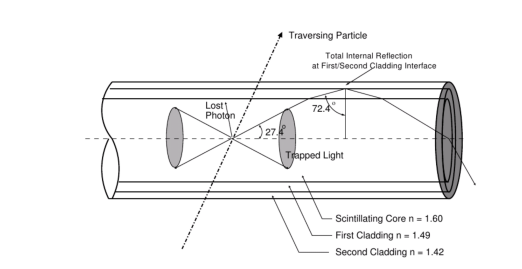
\includegraphics[width=0.8\textwidth]{content/Figures/Quer.PNG}
    \caption{Schematische Darstellung einer Szintillationsfaser mit zwei Ummantelungen. Zusätzlich sind die Kritischen Winkel für die Totalreflexion dargestellt \cite{Collaboration2014}.}
    \label{fig:Totalreflexion}
\end{figure}
In Abbildung~\ref{fig:Totalreflexion} ist eine schematische Darstellung einer Szintillationsfaser mit zwei Ummantelungen dargestellt.
Nach dem Snell'schen Gesetz gilt für die Totalreflexion, dass der Einfallswinkel an der Grenzfläche größer als der kritische Winkel $\theta_c = \arcsin\left(\frac{n_2}{n_1}\right)$ sein muss.
Für den Bereich zwischen den beiden Ummantellungengen ergibt sich  wie in Abbildung~\ref{fig:Totalreflexion} dargestellt $\theta_c = 72.4^\circ$.
Daraus folgt, 
dass ein Photon,
welches durch ein geladenes Teilchen in der Faser Längsache erzeugt wird,
in einem Kegel mit einem Öffnungswinkel von $2\cdot 26.7^\circ$ durch Totalreflexion transportiert wird\cite{Lukas}.

\begin{figure}
    \centering
    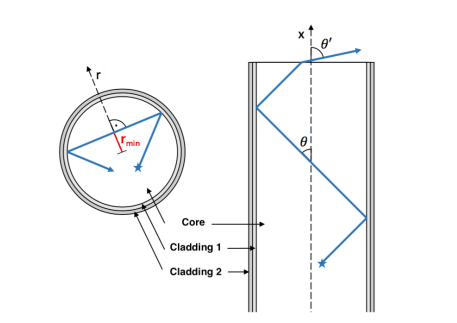
\includegraphics[width=0.8\textwidth]{content/Figures/knickknack.PNG}
    \caption{Schematische Darstellung der Bewegung eines Photons in einer Szintillationsfaser, unter der Annahme, das es sich durch den Kern der Faser bewegt \cite{Anleitung}.}
    \label{fig:knickknack}  
\end{figure}
Unter der Annahme,
dass die Photonen sich durch den Kern der Faser bewegen,
kann die Anzahl der Totalreflexionen $N$ eines Photons berechnet werden durch:
\begin{equation}
    N = \frac{x\tan(\theta)}{2\sqrt{r_\text{core}^2-r_\text{min}^2}}  
\end{equation}
Wobei $x$ die Länge der Faser, $r_\text{core}$ der Radius des Kerns der Faser, $r_\text{min}$ der minimale Abstand des Photons von der Längsachse der Faser und $\theta$ der Winkel zwischen der Längsachse und der Richtung des Photons ist.
Eine Schematische Darstellung der Parameter ist in Abbildung~\ref{fig:knickknack} dargestellt.
Die zurückgelegte Strecke $L$ durch die Faser ergibt sich durch:
\begin{equation}
    L = \frac{x}{\cos(\theta)}.
    \label{eq:1}
\end{equation}

Der Winkel $\theta_\text{refl}$ unter dem das Photon an der Grenzfläche reflektiert wird,
kann geometrisch durch die Abhängigkeit von $r_\text{min}$ und $r_\text{core}$ beschrieben werden durch:
\begin{equation}
    \theta_\text{refl} = \arcsin\left(\sqrt{1 -\frac{r^2_\text{min}}{r^2_\text{core}}}\sin(\theta)\right).    
    \label{eq:2}
\end{equation} 
Es wird deutlich,
das wenn $r_\text{min}$ gegen $r_\text{core}$ geht,
Totalrefelexion schon bei $0^\circ$ auftritt.
Geht $r_\text{min}$ gegen hingegen gegen $0$,
so ist erwartungsgemäß $\theta_\text{refl} = \theta$.

Die Anzahl der Photonen,
welche das Ende der Faser unter dem Winkel $\theta$ und der Entfernung x erreichen,
kann durch die Intensität $I(x,\theta)$ beschrieben werden.
Die Abnahme der Intensität,
kann durch zwei seperierte Effekte beschrieben werden.
Zum einen durch Absorbtionen durch das Material der Faser ($I_\text{core}$).
Dies geschieht durch auftretende von Rayleigh-Streuung, 
welche den Winkel der Photonen so ändert,
dass es nicht mehr zu Totalreflektion kommt.
Zusätzlich kommt es durch verschiedene Effekte zur Absorption der Photonen durch die Faser.
So werden durch die Photonen Phononen angeregt und auch die self-Absorbtion durch die Wavelength Shifter führt zu einer Abnahme der Intensität.

Zum anderen kommt es zu verlusten von Photonen durch Reflektionen an der Grenzfläche zwischen den Materialien.
Die totalre Intensität $I_\text{total}$ kann durch die folgende Formel beschrieben werden:
\begin{equation}
    I_\text{total}(x,\theta) = I_0 \cdot I_\text{core}(x,\theta) \cdot I_\text{refl}(x,\theta).
\end{equation}

In Abhängigkeit von der zurückgelegten Strecke $L$ durch die Faser und der Dämpfungslänge $\lambda$ kann die abnahme der Keren Intebnsität beschrieben werden durch:
\begin{equation}
    I_\text{core}(x,\theta) = \exp{-\frac{L(x,\theta)}{\lambda}}.
\end{equation}
Die Intensität der reflektierten Photonen $I_\text{refl}$ kann durch die Anzahl der Reflektionen $N$ und der zurückgelegten Strecke $L$ beschrieben werden durch:
\begin{equation}
    I_\text{refl}(x,\theta) = I_0\exp{\left(-\frac{L(x,\theta)}{\lambda}-N(x,\theta)\right)}.
\end{equation}
Setzt man hier die Formeln \ref{eq:1} und \ref{eq:2} für $L$ und $N$ ein,
so ergibt sich die folgende Formel für die Intensität der reflektierten Photonen:
\begin{equation}
    I_\text{refl}(x,\theta) = I_0\exp{\left(-\frac{x}{\lambda \cos(\theta)}-\frac{x\tan(\theta)}{2\sqrt{r_\text{core}^2-r_\text{min}^2}}\right)}.
\end{equation}
Woraus sich die effektive Dämpfungslänge $a_\text{eff}$ ergibt durch:
\begin{equation}
    a_\text{eff}(\theta) = \frac{a_0}{\cos(\sigma)} + \frac{\epsilon\tan{\theta}}{2\sqrt{r^2_\text{core}-r^2_\text{min}}} .  
\end{equation}


\subsection{Silicon Photomultiplier}
Silizium-Photomultiplier (SiPMs) werden im SciFi-Tracker eingesetzt, 
um die von den Szintillationsfasern erzeugten Photonen nachzuweisen. 
Dazu sind sie direkt an den Enden der Fasermatten angebracht. 
in SiPM besteht aus einer Matrix vieler einzelner Avalanche-Photodioden-Pixel, 
die im sogenannten Geiger-Modus betrieben werden.

Trifft ein Photon auf ein solches Pixel und wird absorbiert, 
erzeugt es ein Elektron-Loch-Paar. 
Durch das angelegte elektrische Feld werden diese Ladungsträger getrennt und beschleunigt. 
Dabei gewinnen die Elektronen genügend Energie, 
um weitere Elektron-Loch-Paare zu erzeugen. 
Es kommt zu einer lawinenartigen Verstärkung (Avalanche), 
bei der typischerweise etwa ($10^6)$ Elektronen entstehen. D
iese Ladungslawine führt zu einem messbaren Strompuls.

Damit das Pixel nach einem solchen Ereignis wieder empfindlich wird, 
muss die Avalanche gestoppt werden. 
Dies geschieht durch einen in Reihe geschalteten Widerstand, 
der den Strom begrenzt und die Lawine „quencht“. 
Anschließend ist das Pixel wieder bereit, 
ein neues Photon zu detektieren.

Eine zentrale Kenngröße von SiPMs ist die Photodetektionseffizienz (Photon Detection Efficiency, PDE). 
Sie beschreibt das Verhältnis zwischen detektierten und tatsächlich einfallenden Photonen und hängt stark von der Wellenlänge des Lichts ab. 
Im Maximum liegt die PDE bei etwa $43\%$.

Eine weitere wichtige Eigenschaft ist die Dunkelrate (dark count rate), 
also das Signalrauschen, 
das ohne einfallendes Licht entsteht. 
Dieses Rauschen ist temperaturabhängig und wird hauptsächlich durch thermisch erzeugte Ladungsträger verursacht. 
Um diesen Effekt zu minimieren, 
werden die SiPMs im SciFi-Tracker bei einer Temperatur von etwa \SI{-40}{\celsius} betrieben.

Zu beachten ist, 
dass SiPMs keine Information über die Wellenlänge der detektierten Photonen liefern. 
Zudem sind sie so montiert, 
dass sie das gesamte am Faserende austretende Licht integrieren \cite{Anleitung}. 

